\chapter{Ontology design and implementation}
This chapter details the design and the implementation phase of the prompt engineering ontology, starting from an ontology engineering methodology chosen based on specific motivations.\\
In the background chapter, in particular in the sections \textit{"Ontology engineering methodologies"} and \textit{"LOT methodologies"} the main state-of-art ontology engineering methodologies have been illustrated:
\begin{itemize}
    \item \textbf{Methontology}
    \item \textbf{NeOn}
    \item \textbf{eXtreme design}
    \item \textbf{LOT - Linked Open Terms}
\end{itemize}
Additionally, in the section \textit{"Ontology engineering using large language models"} two experimental methodologies were analyzed, including \textbf{NeOnGPT}, which employs large language models. Each methodology has its features and defines a workflow in order to develop successfully an ontology. The choice of the methodology to follow during the design and development phase is based on an analysis of the pros and cons of each, considering not only their features but also the available resources and the related projects provided by each one. \\
In the state-of-the-art study, the most recent and comprehensive methodology is the \textbf{LOT methodology}, which I have decided to choose and according to which the development of the prompt engineering ontology will be carried out. Compared to other methodologies analyzed, this is a recent methodology, introduced in 2022, and has been used in various projects such as the 'Ciudades Abiertas' project \cite{ciudad} for the construction of a set of ontologies used for sharing open data, and the BIMERR project \cite{bimerr}, in which ontologies for sustainable construction were developed \cite{bountouni2021bimerr}, among many others available on the LOT methodology website: \href{https://lot.linkeddata.es/}{https://lot.linkeddata.es/}. The LOT methodology has not only been successfully applied in industrial projects but also in the development of various research ontologies, as seen in the background chapter, as it provides a straightforward and iterative method for designing and developing ontologies. Another reason for choosing this methodology is its ease of learning, as it is inspired by the agile methodology in software development. Moreover, the Linked Open Terms project not only provides very useful examples of ontologies to draw inspiration from but also offers a Github repository \cite{lot_github} with all the necessary resources to be used in the specification of requirements. This last aspect is very important because the main drawback of the other methodologies analyzed is the lack of concrete guidelines and the relevant tools to use, tools that, when mentioned, are often obsolete or inaccessible. This complicates the work of a developer who is approaching ontology engineering for the first time, as he needs to understand the fundamentals of the methodology but also figures out which development, validation, and testing software to use. The LOT methodology, thanks not only to the numerous available resources but also to the clear and precise description of the method and the recent tools to be used, resolves these issues and simplifies the developer's work. The LOT methodology has an inherently iterative nature and is oriented towards the publication of ontologies according to the FAIR principles \cite{fair_eu} (Findable, Accessible, Interoperable, Reusable) including specific recommendations, tips and potential
tools that can be helpful to ontology developers moreover the methodology extends the state-of-art methodologies like NeOn and Methontology with a modern approach.
The LOT methodology was preferred over recently introduced techniques that involve the use of large language models in the construction of ontologies and knowledge graphs, such as NeOnGPT. Although these techniques automate the work of the ontology engineer by using large language models, they are computationally expensive and require numerous checks to verify the syntactic and semantic correctness of the produced artifact. Another downside is the lack of actual ontology projects implemented using large language models, as these are very recent techniques that have not been tested on real projects but only on experimental cases.\\
In the following sections, the application of the LOT methodology to the design and implementation of the prompt engineering ontology will be described, following the workflow outlined and described in the background chapter.

\newpage

\section{Ontology requirements specification}
The LOT methodology includes six mandatory phases (plus one optional) in the ontology requirement specification. At the end of each phase, a document is produced containing the analyzed aspect of the specifications, as shown in the following figure:
\begin{figure}[H]
    \centering
    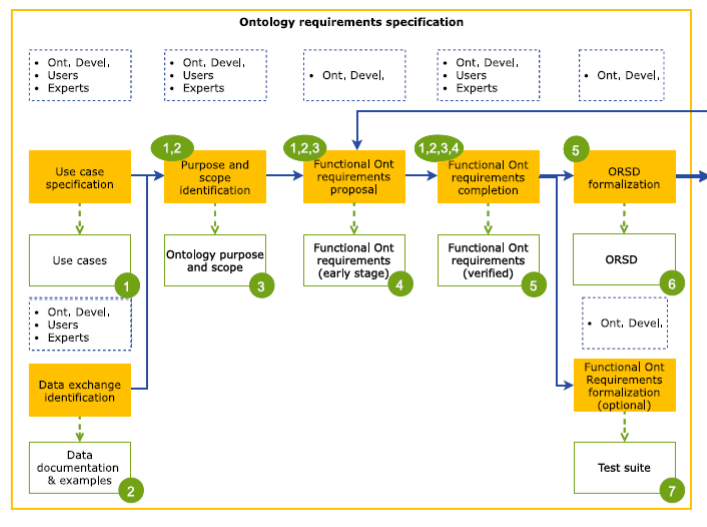
\includegraphics[width=0.9\linewidth]{Figures/fig_13.PNG}
    \caption{Ontology requirements specification workflow}
    \label{fig:enter-label}
\end{figure}
In detail the phases are the following:
\begin{enumerate}
    \item Use case specification
    \item Data exchange identification
    \item Purpose and scope identification
    \item Functional ontology requirements proposal
    \item Functional ontology requirements completion
    \item ORSD formalization 
    \item Functional ontology requirements formalization (optional)
\end{enumerate}

\subsection{Use case specification}
The first step in the design of the prompt engineering ontology is the use case specification, this phase involves domain experts, ontology developers and users and it has the goal to imagine and specify how the ontology can be used in real life by real users. Taking into account the domain, the possible use and the possible users I decided to specify ten use cases. Each use case has a name, a description, a list of actors and a flow.\\

\textbf{Use case 1:}
\begin{itemize}
    \item Name: Optimizing LLM Responses
    \item Description: Researchers use PEO ontology to design optimized prompts that improve LLM response quality.
    \item Actors: Researcher, PEO ontology, LLM.
    \item Flow: The researcher uses the ontology to identify appropriate prompts for different types of tasks creating a set of selected prompts. Selected prompts are given as input to the large language model and responses are evaluated according to specific metrics on consistency, completeness and quality decided by the researcher.
\end{itemize}
The use case is aimed at researchers in the field of artificial intelligence and large language models who want to use the ontology as a support for creating prompts through the various techniques represented. The prompts can be input into one or more large language models (possibly selected from those represented in the ontology), and the responses obtained are evaluated according to metrics chosen by the researchers.\\

\textbf{Use case 2:}
\begin{itemize}
    \item Name: Bias analysis
    \item Description: Researchers use PEO ontology to generate responses and detect bias in large language models considered.
    \item Actors: Researcher, PEO ontology, LLMs
    \item Flow: The researcher uses the ontology to generate prompts on sensitive topics (gender, ethnicity …) and prompts are tested on one or more large language models. Responses are collected using bias and fairness metrics and results are collected in order to improve prompts and considered models. 
\end{itemize}
The use case is aimed at researchers who may want to understand the presence of bias in a selected large language model, such as gender bias. To detect the presence or absence of these biases, they generate prompts on sensitive topics using techniques like zero-shot prompting or chain-of-thoughts. The prompting techniques represented in the ontology can be applied for various purposes in text generation. \\

\textbf{Use case 3:}
\begin{itemize}
    \item Name: Code generation
    \item Description: Developers use prompt engineering techniques applied to a chosen large language model to generate source code in a specific programming language for a specific task.
    \item Actors: Developers, PEO ontology, LLM
    \item Flow: The developer is working on an Android application written in Java and needs code to control the actions on a button. Using the ontology, he chooses the most appropriate prompt engineering technique and applies it to the creation of the prompt to a large language model of his choice,  resulting in Java code as output. The code is tested and integrated into the application. 
\end{itemize}
This use case is aimed at software developers who need assistance in generating a piece of source code in a programming language. The developer can use techniques like few-shot prompting or Auto-CoT to generate code using a large language model selected from those represented in the ontology. \\ 

\textbf{Use case 4:}
\begin{itemize}
    \item Name: Prompt engineering lesson
    \item Description: The teacher uses PEO ontology to teach prompt engineering techniques exploring different techniques and prompt described. 
    \item Actors: Teacher, students, PEO ontology. 
    \item Flow: The teacher opens the ontology and shows with proper explanation different prompt engineering techniques represented in the ontology.
\end{itemize}
The prompt engineering ontology can be used for learning prompt engineering techniques, thanks to the classes and relationships present, and serves as a valuable support for a computer science instructor during lessons.\\

\textbf{Use case 5:}
\begin{itemize}
    \item Name: Large language models lesson
    \item Description: The teacher uses PEO ontology to teach different large language models available.
    \item Actors: Teacher, students, PEO ontology.
    \item Flow: The teacher opens the ontology and shows with proper explanation different large language models represented in the ontology. 
\end{itemize}
Similar to the previous use case, the ontology of prompt engineering represents state-of-the-art large language models and their relationships. This representation can be useful for an instructor to explain large language models during lessons. \\

\textbf{Use case 6:}
\begin{itemize}
    \item Name: Social media content creation
    \item Description: The content creator uses PEO ontology to generate prompts that optimize the creation of articles, social media posts and other textual content.
    \item Actors:  Content creator, PEO ontology, LLM
    \item Flow: The content creator opens the ontology and chooses the appropriate technique in order to generate text for a post on social media using a specific large language model. The content creator adapts the response according to his target.
\end{itemize}
This use case is aimed at content creators and copywriters who want to create textual content for major social platforms and need support in writing effective content. They can select one of the prompt engineering techniques represented, such as Retrieval Augmented Generation (RAG) or few-shot prompting and by starting from examples of previous articles or posts, they can create a prompt capable of generating text that meets the content creator's request.\\

\textbf{Use case 7:}
\begin{itemize}
    \item Name: Image generation
    \item Description: The content creator uses PEO ontology to create a prompt to be given as input to a specific large language model capable of generating an image.
    \item Actors: Content creator, PEO ontology, LLM.
    \item Flow: The content creator wants to create an AI-generated image for a video and he uses the ontology to choose the best large language models able to generate image, he chooses the prompt engineering technique to create the prompt in order to generate image. He watches the output and he continues to use the ontology to generate prompts in order to refine the image.
\end{itemize}
In the PEO ontology, not only are techniques for generating text represented, but there are also techniques for generating images using generative models like DALL-E or Midjourney. This allows a user to utilize the ontology not only to understand which model to use but also to choose the appropriate technique for writing the prompt to obtain an image that meets their preferences.\\

\textbf{Use case 8:}
\begin{itemize}
    \item Name: Prompt engineering experiments
    \item Description: Students use PEO ontology to explore and create effective prompts to improve language model responses.
    \item Actors: Students, PEO ontology, LLM.
    \item Flow: Students explore the ontology in order to understand different prompting techniques applying them to a chosen large language model.
\end{itemize}
As seen in the previous use cases, the ontology can be used for educational purposes by instructors as a support for explaining prompt engineering techniques and large language models. At the same time, it can be used by students to clearly learn these concepts. In this particular case, students learn and experiment with various techniques represented in the ontology by writing different prompts using a large language model like ChatGPT.\\

\textbf{Use case 9:}
\begin{itemize}
    \item Name: Large language models learning
    \item Description: Students use PEO ontology to learn different types of large language models.
    \item Actors: Students, PEO ontology
    \item Flow: Students explore different large language models represented in the ontology and the relationships among them, learning all the features of each large language model.
\end{itemize}
This use case is similar to the previous one, where students use the ontology to learn about state-of-the-art large language models by exploring their relationships with tasks and the prompt engineering techniques represented.\\

\textbf{Use case 10:}
\begin{itemize}
    \item Name: Explanation computer science topics
    \item Description: Student wants to generate a prompt using PEO ontology in order to explain a computer science topic.
    \item Actors: Student, PEO ontology, LLM
    \item Flow: The student uses the ontology to choose the most appropriate prompt engineering technique in order to generate using large language models. The student reads the obtained LLM response and can create a new prompt using another technique represented in the ontology.
\end{itemize}
In the two previous use cases, the ontology is used as a support to learn concepts related to large language models and prompt engineering. However, it is also possible to use the ontology to generate prompts using techniques like zero-shot prompting or ReAct Prompting, in order to explain a specific topic with an LLM represented in the ontology.\\
The use cases have been designed with the idea of creating an ontology that is not just an encyclopedic resource for students and teachers but also a practical tool for professionals and researchers in writing effective prompts suited to their goals. The narrative description of each use case flow helps to embody each user, aiming to better understand their needs and requirements that the prompt engineering ontology will need to meet.

\subsection{Data exchange identification}
The goal of the data exchange identification activity is to provide the necessary documentation
about the domain to be modeled. Essentially, this phase involves gathering heterogeneous sources of information, such as scientific papers, websites, datasets, and similar existing ontologies. The LOT methodology does not provide a clear indication of how to represent this documentation, so for simplicity and clarity, I have decided to collect the links to the scientific papers and web pages containing information to be represented in the ontology in a dedicated file. The list of papers chosen as a source for the prompt engineering ontology is as follows:
\begin{itemize}
\item A Systematic Survey of Prompt Engineering in Large Language Models: Techniques and Applications \cite{sahoo2024systematic}

\item Pre-train, Prompt, and Predict: A Systematic Survey
of Prompting Methods in Natural Language Processing \cite{liu2023pre}

\item A Survey of Large Language Models \cite{zhao2023survey}

\item Investigating Prompt Engineering in Diffusion
Models \cite{witteveen2022investigating}

\item A Survey on Large Language Models: Applications,
Challenges, Limitations, and Practical Usage \cite{hadi2023survey}

\item Large Language Models: A Survey \cite{minaee2024large}
\end{itemize}
The list of website chosen is the following:
\begin{itemize}
    \item \href{https://www.promptingguide.ai/}{Prompting Guide}
    
    \item \href{https://github.com/Hannibal046/Awesome-LLM}{Awesome-LLM}

    \item \href{https://llmmodels.org/}{List of LLMs}

    \item \href{https://learnprompting.org/}{Learn prompting}
\end{itemize}
Unfortunately, the resources found and deemed useful for developing the ontology are not many, as the topic is very recent. Additionally, no datasets containing prompts generated with specific techniques were found, only datasets with generic prompts for text generation, such as the dataset available on Huggingface, "awesome-gpt-prompts" \cite{awesome_gpt}, and the "diffusion-db" dataset \cite{diffusion_db}, which, although it contains over 16 million prompts for image generation, does not specify the prompt engineering technique used.

\subsection{Purpose and scope identification}
From use cases and the domain documentation provided in the data exchange identification task, in this phase there is the specification of the purpose: what is the objective of the prompt engineering ontology and the specification of the scope of the ontology: what it is going to be represented in the ontology. The PEO ontology aims to formalize knowledge about the creation and various types of prompts for the different large language models (LLMs) available by making it accessible to both experienced and less experienced users. This is the purpose of the PEO ontology.
The PEO ontology is going to cover:
\begin{itemize}
    \item Large language models (LLMs) available to users
    \item Prompt engineering techniques
    \item Task that can be solved using a large language model
    \item Examples of prompts specific to the large language model
\end{itemize}
This is the scope of the PEO ontology.
In general, the goal of the project and the ontology is to create a resource accessible to everyone on a recently introduced topic, for which there are not many available resources. This resource aims to support not only the learning but also the application of prompt engineering techniques and large language models.

\subsection{Functional ontology requirements specification}
The LOT methodology provides for the specification of requirements in one of three ways: through competency questions, through natural language statements, or through tabular information containing concepts, relationships, and attributes. As seen in the background chapter, competency questions are widely used in ontology engineering and allow for clearly expressing the functional requirements of an ontology. In the case of the prompt engineering ontology, based on the use cases and the purpose and scope identification described earlier, I have identified eighteen competency questions, which are:
\begin{itemize}
    \item \textbf{CQ1:} What is prompt engineering?

    \item \textbf{CQ2:} What is a prompt?

    \item \textbf{CQ3:} What are prompting techniques?

    \item \textbf{CQ4:} What are image prompting techniques?

    \item \textbf{CQ5:} What are code prompting techniques?

    \item \textbf{CQ6:} Which task does a prompt solve?

    \item \textbf{CQ7:} Which prompts are generated using a prompting technique?

    \item \textbf{CQ8:} What are responses of each prompt?

    \item \textbf{CQ9:} What are possible tasks?

    \item \textbf{CQ10:} Which tasks are related to the text?

    \item \textbf{CQ11:} What chats does each large language model have?

    \item \textbf{CQ12:} What is a large language model?

    \item \textbf{CQ13:} What types of large language models are available?

    \item \textbf{CQ14:} What are the available versions of each large language model?

    \item \textbf{CQ15:} What are large language models architectures?

    \item \textbf{CQ16:} What are large language models capabilities?

    \item \textbf{CQ17:} What companies develop large language models?

    \item \textbf{CQ18:} What is the first version of each large language model developed by each company?
\end{itemize}
Competency questions are saved into an excel file, the template is available in the \href{https://github.com/oeg-upm/LOT-resources}{official Github repository}. The Excel file not only contains the competency questions but also specifies for each one: the identifier, the domain, the answer, the status (Proposed, Accepted, Rejected, Pending, Deprecated), comments, and priority (high, medium, and low). All the competency questions have a high priority, as they form the foundation for the design of the prompt engineering ontology, covering both the prompt engineering and large language models domain in order to produce a complete ontology.

\subsection{ORSD formalization}
The final step in the specification of ontology requirements is the writing of the ORSD (Ontology Requirements Specification Document), a document that gathers the main information defined in the previous phase, namely the purpose and scope of the ontology, the use cases, the functional requirements (expressed through competency questions), and the non-functional requirements. First introduced by the NeOn methodology, which I discussed in the previous chapter, the writing of the ORSD follows a specific sequence of tasks to ensure its correctness and completeness. The workflow is described in the paper \textit{How to Write and Use the Ontology Requirements Specification Document}\cite{suarez2009write} and involves a sequence of eight tasks, starting from ontological needs: 
\begin{enumerate}
    \item Identify purpose, scope and implementation language.
    \item Identify intended end-users
    \item Identify intended uses
    \item Identify requirements
    \item Group requirements
    \item Validate the set of requirements
    \item Prioritize requirements
    \item Extract terminology and its frequency
\end{enumerate}

The LOT methodology adopted the ORSD introduced by NeOn but adapted it with appropriate modifications. Unlike NeOn, it does not consider the "user" field as mandatory, and the glossary of terms is built starting from the competency questions.\\
In writing the ORSD for the PEO ontology, the \href{https://github.com/oeg-upm/LOT-resources/tree/master/templates%20for%20ORSD}{template from the official LOT repository}\cite{template_orsd} was used. 
In the document, the information obtained in the previous phases has been included, namely purpose and scope identification and ontology requirements in the form of competency questions. Additionally, further information that emerged during the requirements gathering phase has also been included:
\begin{itemize}
    \item Implementation language 
    \item Intended End-Users 
    \item Intended Uses
    \item Non-Functional Requirements
\end{itemize}
In detail the implementation language is OWL (Ontology Web Language) using the Protegé software\cite{protege_sw}, an open-source popular software released by Stanford univerisity. As seen in the use case the intended end-users of the prompt engineering ontology are:
\begin{itemize}
    \item Researchers in the field of artificial intelligence using LLMs for research purpose.
    \item Software engineers and developers.
    \item Educators and trainers teaching students or professionals about AI and prompt engineering, using the ontology as a learning and instructional tool.
    \item Content Creators using LLMs for generating content.
    \item Undergraduate and high school students learning about AI, LLMs and prompt engineering, using the ontology to understand core concepts and experiment with language models.
\end{itemize}
Starting from the use cases, it is possible to easily deduce the intended uses:
\begin{itemize}
    \item Prompt generation
    \item Large language models learning
    \item Prompt engineering learning
    \item Prompt generation for a specific task
\end{itemize}
Regarding non-functional requirements, the characteristics, qualities and general aspects not related to the ontology content that the ontology should satisfy, I have identified six non-functional requirements:
\begin{itemize}
    \item \textbf{NFR1:} The ontology must be easy to use.
    \item \textbf{NFR2:} The ontology must cover most used LLMs.
    \item \textbf{NFR3:} The ontology must cover modern prompt engineering techniques.
    \item \textbf{NFR4:} The ontology must have exhaustive documentation.
    \item \textbf{NFR5:} The ontology must be easy to update. 
    \item \textbf{NFR6:} The ontology must cover most popular tasks. 
\end{itemize}
Those non-functional requirements match with the desired properties of the prompt engineering ontology, since the ontology will be used by both expert users (researchers, developers) and less experienced users (students), it must be easy to use, meaning it should include classes, relations, and entities that are easily understandable by everyone. Given that the ontology must represent prompt engineering techniques and LLMs, it should cover the most up-to-date techniques and models, as outdated ones would render it useless. The same applies to the tasks: the ontology must represent the main tasks that large language models can be applied to and where prompt engineering techniques can be used. Since the domain represented by the ontology is continuously and rapidly evolving, the ontology must be easily updatable and well-documented to simplify the work for other developers.


\newpage
\section{Ontology implementation}





\begin{figure}[H]
    \centering
    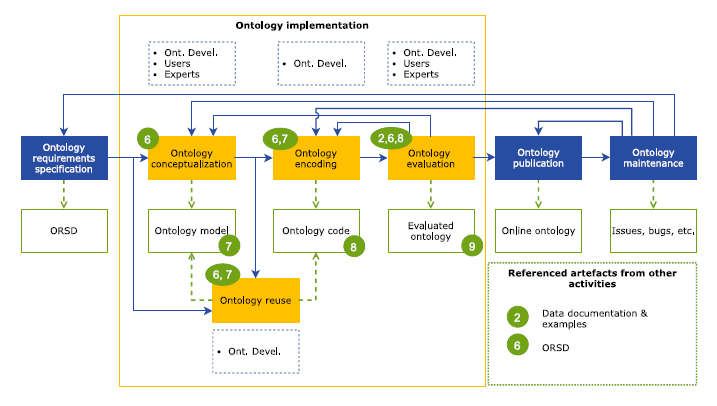
\includegraphics[width=0.9\linewidth]{Figures/fig_14.png}
    \caption{Ontology implementation workflow}
    \label{fig:enter-label}
\end{figure}

\newpage
\section{Ontology publication}